\documentclass[12pt]{beamer}
\usetheme{default}
\usecolortheme{beetle}

\usepackage[utf8]{inputenc}
\usepackage[english]{babel}
\usepackage{amsmath}
\usepackage{amsfonts}
\usepackage{amssymb}
\usepackage{graphicx}
\usepackage{tikz}
\usepackage{listings}

\title{Graph Data - Modelling and Quering}
\subtitle{with Neo4j and Cypher}
\author[I.Feuerstein]{Iryna Feuerstein}
\institute[ODSC]{Open Data Science Conference}
\titlegraphic{
\includegraphics[height=0.6cm]{pd_logo.png}}
\logo{
\includegraphics[height=0.7cm]{logo.png}\vspace{230pt}}
\date{12 October 2017}
\setbeamertemplate{background}
{
\includegraphics[width=\paperwidth,height=\paperheight,keepaspectratio]{background.png}}
\begin{document}
    
    \begin{frame}
        \frametitle{Introduction}
        Please find two other learning partners, 
        \begin{itemize}
            \item form a standing group and 
            \item tell them what you already know about \begin{itemize}
                \item graphs, 
                \item graph databases and 
                \item Neo4j.
            \end{itemize}
        \end{itemize}
    \end{frame}
    
    \maketitle
    
    \begin{frame}
        \frametitle{Agenda}
        \tableofcontents
    \end{frame}
    
    \section{What are graphs?}
    \subsection{Definition}
    
    \begin{frame}
        \frametitle{Graph}
        \begin{Definition}
            \emph{Graph} is an ordered pair \(G = \left(V,E\right)\) comprising a set \(V\) of \emph{vertices}, \emph{nodes} or \emph{points} together with a set \(E\) of \emph{edges}, \emph{arcs} or \emph{lines}, which are 2-element subsets of V.\footnotemark
        \end{Definition}
        \pause
        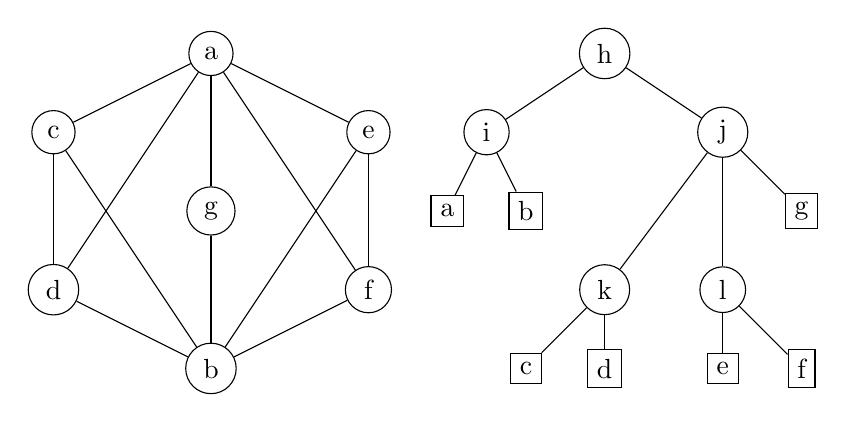
\begin{tikzpicture}
        \node[draw, circle] (a) at (3,4){a};
        \node[draw, circle] (b) at (3,0){b};
        \node[draw, circle] (c) at (1,3){c};
        \node[draw, circle] (d) at (1,1){d};
        \node[draw, circle] (e) at (5,3){e};
        \node[draw, circle] (f) at (5,1){f};
        \node[draw, circle] (g) at (3,2){g};
        \draw[-] (a)--(c);
        \draw[-] (a)--(d);
        \draw[-] (a)--(e);
        \draw[-] (a)--(f);
        \draw[-] (a)--(g);
        \draw[-] (b)--(c);
        \draw[-] (b)--(d);
        \draw[-] (b)--(e);
        \draw[-] (b)--(f);
        \draw[-] (b)--(g);
        \draw[-] (c)--(d);
        \draw[-] (e)--(f);
        
        \node[draw, circle](root) at (8,4){h};
        \node[draw, circle](ab) at (6.5,3){i};
        \node[draw, circle](root-g) at (9.5,3){j};
        \node[draw, circle](cd) at (8,1){k};
        \node[draw, circle](ef) at (9.5,1){l};
        \node[draw](a) at (6,2) {a};
        \node[draw](b) at (7,2) {b};
        \node[draw](c) at (7,0) {c};
        \node[draw](d) at (8,0) {d};
        \node[draw](e) at (9.5,0) {e};
        \node[draw](f) at (10.5,0) {f};
        \node[draw](g) at (10.5,2) {g};
        \draw [-] (root)--(ab);
        \draw [-] (root)--(root-g);
        \draw [-] (ab)--(a);
        \draw [-] (ab)--(b);
        \draw [-] (root-g)--(cd);
        \draw [-] (root-g)--(ef);
        \draw [-] (root-g)--(g);
        \draw [-] (cd)--(c);
        \draw [-] (cd)--(d);
        \draw [-] (ef)--(e);
        \draw [-] (ef)--(f);
        \end{tikzpicture}
        \footnotetext{\url{en.wikipedia.org/wiki/Graph_(discrete_mathematics)}}
    \end{frame}
    
    \subsection{Typical use cases}
    \begin{frame}
        \frametitle{Use Cases}
        \begin{itemize}
            \pause
            \item Networks
            \begin{itemize}
                \item Social networks\\[3mm]
                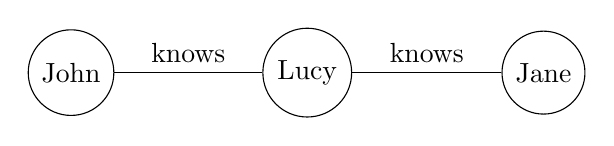
\begin{tikzpicture}
                \node[draw, circle](john) at (0,0){John};
                \node[draw, circle](lucy) at (3,0){Lucy};
                \node[draw, circle](jane) at (6,0){Jane};
                \path (john) edge node [above] {knows} (lucy);
                \path (lucy) edge node [above] {knows} (jane);
                \end{tikzpicture}
                \pause
                \item Computer networks\\[3mm]
                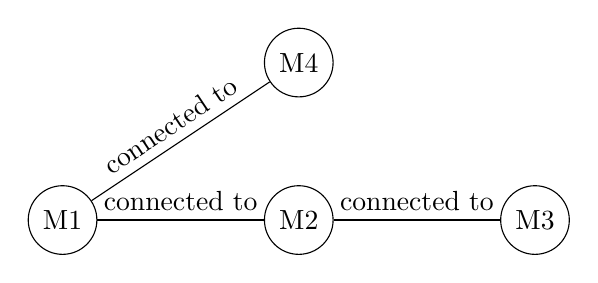
\begin{tikzpicture}
                \node[draw, circle](m1) at (0,0){M1};
                \node[draw, circle](m2) at (3,0){M2};
                \node[draw, circle](m3) at (6,0){M3};
                \node[draw, circle](m4) at (3,2){M4};
                \path (m1) edge node [above] {connected to} (m2);
                \path (m2) edge node [above] {connected to} (m3);
                \path (m1) edge node [pos=0.5, sloped, above] {connected to} (m4);
                
                \end{tikzpicture}
            \end{itemize}
        \end{itemize}
    \end{frame}
    
    \begin{frame}
        \frametitle{Use Cases}
        \begin{itemize}
            \item Networks
            \begin{itemize}
                \item Transport networks\\[3mm]
                
                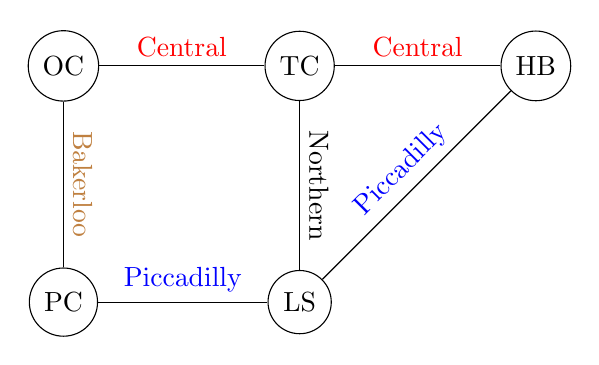
\begin{tikzpicture}
                \node[draw, circle](m1) at (0,3){OC};
                \node[draw, circle](m2) at (3,3){TC};
                \node[draw, circle](m3) at (6,3){HB};
                \node[draw, circle](m4) at (3,0){LS};
                \node[draw, circle](m5) at (0,0){PC};
                \path (m1) edge node [above, red] {Central} (m2);
                \path (m2) edge node [above, red] {Central} (m3);
                \path (m3) edge node [pos=0.5, sloped, above, blue] {Piccadilly} (m4);
                \path (m4) edge node [pos=0.5, sloped, above, blue] {Piccadilly} (m5);
                \path (m1) edge node [pos=0.5, sloped, above, brown] {Bakerloo} (m5);
                \path (m2) edge node [pos=0.5, sloped, above] {Northern} (m4);
                \end{tikzpicture}\\
                OC = Oxford Circus\\
                TC = Tottenham Court Road\\
                HB = Holborn\\
                LS = Leicester Square\\
                PC = Piccadilly Circus
            \end{itemize}
        \end{itemize}
    \end{frame}
    
    \subsection{Not so typical use cases}
    \begin{frame}
        \frametitle{Use Cases}
        \begin{itemize}
            \item Natural Language Processing\\[3mm]
            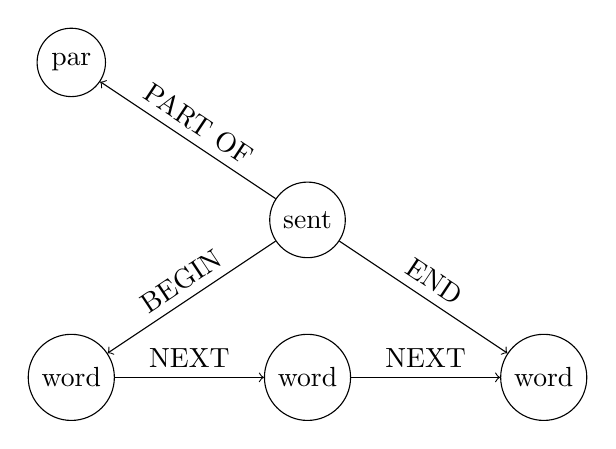
\begin{tikzpicture}
            \node[draw, circle](w1) at (0,0){word};
            \node[draw, circle](w2) at (3,0){word};
            \node[draw, circle](w3) at (6,0){word};
            \node[draw, circle](s) at (3,2){sent};
            \node[draw, circle](p) at (0,4){par};
            \path (w1) edge[->] node [above] {NEXT} (w2);
            \path (w2) edge[->] node [above] {NEXT} (w3);
            \path (s) edge[->] node [sloped, above] {BEGIN} (w1);
            \path (s) edge[->] node [sloped, above] {END} (w3);
            \path (s) edge[->] node [sloped, above] {PART OF} (p);
            \end{tikzpicture}
        \end{itemize}
    \end{frame}
    
    \begin{frame}
        \frametitle{Use Cases}
        \begin{itemize}
            \item Document management\\[2mm]
            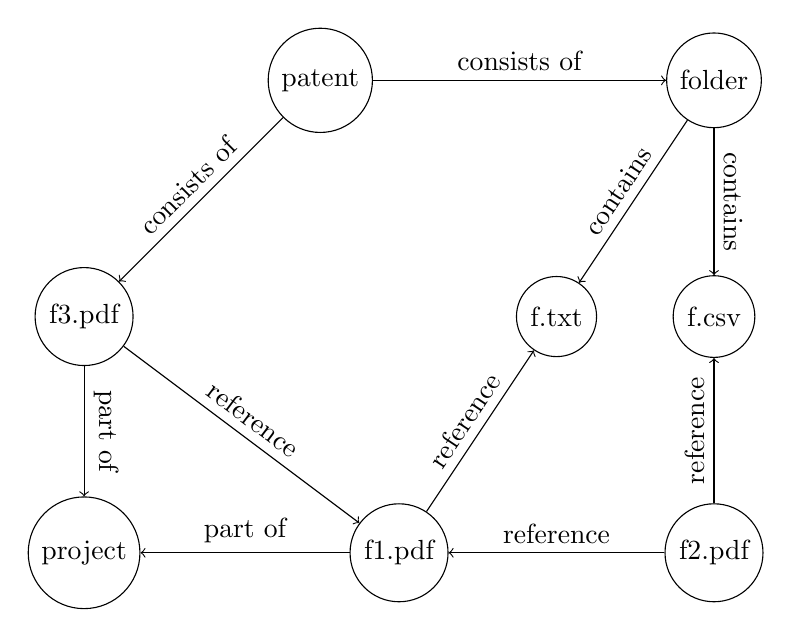
\begin{tikzpicture}
            \node[draw, circle](pr) at (0,0){project};
            \node[draw, circle](f1) at (4,0){f1.pdf};
            \node[draw, circle](f2) at (8,0){f2.pdf};
            \node[draw, circle](f3) at (0,3){f3.pdf};
            \node[draw, circle](txt) at (6,3){f.txt};
            \node[draw, circle](csv) at (8,3){f.csv};
            \node[draw, circle](pt) at (3,6){patent};
            \node[draw, circle](f) at (8,6){folder};
            \path (f1) edge[->] node [above] {part of} (pr);
            \path (f2) edge[->] node [above] {reference} (f1);
            \path (f3) edge[->] node [sloped, above] {part of} (pr);
            \path (f3) edge[->] node [sloped, above] {reference} (f1);
            \path (f1) edge[->] node [sloped, above] {reference} (txt);
            \path (f2) edge[->] node [sloped, above] {reference} (csv);
            \path (pt) edge[->] node [sloped, above] {consists of} (f3);
            \path (pt) edge[->] node [sloped, above] {consists of} (f);
            \path (f) edge[->] node [sloped, above] {contains} (txt);
            \path (f) edge[->] node [sloped, above] {contains} (csv);
            \end{tikzpicture}
        \end{itemize}
    \end{frame}
    
    \begin{frame}
        \frametitle{Use Cases}
        \begin{itemize}
            \item Biochemistry / Genomics\\[2mm]
            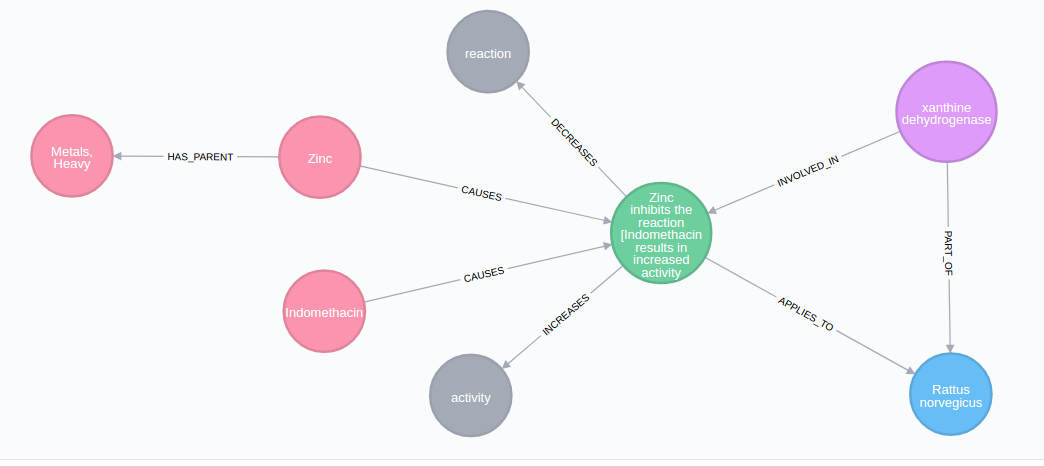
\includegraphics[width=0.9\textwidth]{genomics.png}
        \end{itemize}
        \footnotetext{\url{http://ctdbase.org/}}
    \end{frame}
        
    \section{Starting with Neo4j and Cypher}
    \subsection{Starting the database}
    \begin{frame}
        \frametitle{Installation}
        \begin{itemize}
            \item Find the right installation file for your OS at \url{neo4j-training-files/neo4j} on the flash drive and install the software.
            \pause
            \item Copy both JAR-files from the \url{neo4j-training-files/plugins} directory into \url{NEO4J_HOME/plugins} directory of your Neo4j installation.
            \pause
            \item Replace the \url{NEO4J_HOME/conf/neo4j.conf} configuration file with the one found on the flash drive at \url{neo4j-training-files/conf/neo4j.conf}.
            \pause
            \item Copy the \url{neo4j-training-files/data/odsc.db} folder into your \url{NEO4J_HOME/data/databases/} directory
        \end{itemize}
    \end{frame}
    
    \begin{frame}
        \frametitle{Starting Neo4j}
        \begin{itemize}
            \item Start the database with\\
            \url{NEO4J_HOME/bin/neo4j} \url{start}
            \pause
            \item Go to \url{http://localhost:7474} within you browser
        \end{itemize}
    \end{frame}
    
    \subsection{Brief look at the configuration}
    \begin{frame}
        \frametitle{Demonstration}
        \begin{block}{Important configuration entries}
            dbms.active\_database=odsc.db\\
            dbms.security.auth\_enabled=false\\
            dbms.security.procedures.unrestricted=algo.*,apoc.*\\
            apoc.import.file.enabled=true
        \end{block}
    \end{frame}
    
    \subsection{CRUD operations with Cypher}
    \subsection{Node operations}
    \begin{frame}
        \frametitle{Live coding session}
        \begin{itemize}
            \item create node\\
            CREATE (c:Chemical \{name: 'Helium'\}) RETURN c
            \item update node\\
            MERGE (c:Chemical \{name: 'Helium'\}) SET c.symbol = 'He' RETURN c
            \item delete node 
            \begin{itemize}
                \item without relations\\
                MATCH (c:Chemical \{name:'Helium'\}) DELETE c\\
                MATCH (c:Chemical)\\
                \hspace{1cm} WHERE c.name = 'Helium'\\
                \hspace{1cm} DELETE c
                \item with existing relations\\
                MATCH (c:Chemical \{name:'Helium'\})\\
                \hspace{1cm} DETACH DELETE c\\
            \end{itemize}
        \end{itemize}
    \end{frame}
    
    \subsection{Relation operations}
    \begin{frame}
        \frametitle{Live coding session}
        \begin{itemize}
            \item create relation\\
            \begin{itemize}
                \item between new nodes\\
                CREATE (c:Chemical {chemicalName:'Helium'})-[:BELONGS\_TO]->(g:ChemicalGroup {groupName:'Noble gases'}) RETURN c,g
                \item between existing nodes\\
                MATCH (g:ChemicalGroup {groupName:'Noble gases'}), (p:ChemicalGroup {groupName:'Gases'})
                CREATE (g)-[:HAS\_PARENT]->(p) RETURN g,p
            \end{itemize}
            \item update relation\\
            MATCH ()-[r:BELONGS\_TO]-() SET r.updateTime = timestamp() RETURN r\\
            \item delete relation\\
            MATCH ()-[r:BELONGS\_TO]-() DELETE r
        \end{itemize}
    \end{frame}
    
    \section{Quering for paths and patterns}
    \begin{frame}
        \frametitle{Live coding session}
        Examples:
        \begin{itemize}
            \item MATCH (g:Gene) WHERE g.geneSymbol = 'CTSD' RETURN g
            \item MATCH (g:Gene)<-[:ASSOCIATED\_WITH]-(d:Disease) WHERE g.geneSymbol = 'CTSD' RETURN g, d
            \item MATCH (g:Gene)<-[:ASSOCIATED\_WITH]-(d:Disease) WHERE g.geneSymbol = 'CTSD' RETURN g, count(d)
            \item MATCH (g:Gene)<-[:ASSOCIATED\_WITH]-(d:Disease) WITH g, count(d) as diseases WHERE diseases > 50 RETURN g.geneName, g.geneSymbol, diseases ORDER BY diseases DESC\\
            \item MATCH (g:Gene)<-[:ASSOCIATED\_WITH]-(d:Disease)-[:ASSOCIATED\_WITH]-(otherGene:Gene) WHERE g.geneSymbol = 'CTSD' AND d.diseaseName = 'Osteoarthritis' RETURN otherGene.geneName, otherGene.geneSymbol
        \end{itemize}
    \end{frame}
    
    \begin{frame}
        \frametitle{Live coding session}
        \begin{itemize}
            \item MATCH p = (c:Chemical)-[*2]-(d:Disease) where d.diseaseName STARTS WITH 'Osteo' RETURN p LIMIT 20
            \item MATCH (c:Chemical)<-[:HAS\_PARENT*3..4]-(descendant:Chemical) 
            WITH c, count(descendant) AS descendants , collect(descendant.chemicalName) as names ORDER BY descendants DESC LIMIT 10
            RETURN c.chemicalName, names[1..10], descendants
            \item MATCH (c:Chemical) WHERE c.chemicalName = 'Zinc Acetate'
            MATCH (d:Disease) WHERE d.diseaseName = 'Alzheimer Disease' 
            MATCH p = (c)-[*1..3]-(d)
            RETURN p LIMIT 20
            \item MATCH (c:Chemical {chemicalName:'Zinc Acetate'}), (d:Disease {diseaseName:'Alzheimer Disease'})
            MATCH path = allShortestPaths( (c)-[*..3]-(d) )
            RETURN path
        \end{itemize}
    \end{frame}
    
    \section{Using graph algorithms}
    \begin{frame}
        \frametitle{Calling procedures}
        \begin{itemize}
            \item CALL db.schema
            \item CALL dbms.procedures
            \item call dbms.functions
            \item CALL apoc.help('dijkstra')
        \end{itemize}
    \end{frame}
    
    \subsection{apoc library}
    \begin{frame}
        \frametitle{Live coding session}
        \begin{Definition}
            In a connected graph, the normalized closeness centrality (or closeness) of a node is the average length of the shortest path between the node and all other nodes in the graph. Thus the more central a node is, the closer it is to all other nodes.\footnotemark
        \end{Definition}
        \begin{block}{Closeness Centrality Example}
            MATCH (node:Chemical)
            WHERE node.chemicalName CONTAINS 'Vitamin'
            WITH collect(node) AS nodes
            CALL apoc.algo.closeness(['HAS\_PARENT'],nodes,'BOTH') YIELD node, score
            RETURN node, score
            ORDER BY score DESC
        \end{block}
        \footnotetext{\url{en.wikipedia.org/wiki/Centrality\#Closeness_centrality}}
    \end{frame}
    
    \begin{frame}
        \frametitle{Live coding session}
        \begin{Definition}
            Betweenness centrality quantifies the number of times a node acts as a bridge along the shortest path between two other nodes.\footnotemark
        \end{Definition}
        \begin{block}{Betweenness Centrality Example}
            MATCH (node:Disease)
            WHERE node.diseaseName CONTAINS 'deficiency'
            WITH collect(node) AS nodes
            CALL apoc.algo.betweenness(['HAS\_PARENT'],nodes,'BOTH') YIELD node, score
            RETURN node.diseaseName, score
            ORDER BY score DESC LIMIT 10
        \end{block}
        \footnotetext{\url{en.wikipedia.org/wiki/Centrality\#Betweenness_centrality}}
    \end{frame}
    
    \subsection{algo library}
    \begin{frame}
        \frametitle{Live coding session}
        \begin{block}{PageRank example}
            call algo.pageRank.stream('InteractionType', 'HAS\_PARENT',{iterations:20}) YIELD node, score
            WITH * ORDER BY score DESC LIMIT 5
            RETURN node.typeName, node.code, score;
        \end{block}
    \end{frame}
    
    \section{Importing data}
    \subsection{Basic loading command}
    \subsection{Performance issues and dealing with big data}
    
    
    \section{Refactoring graph data model}
    \begin{frame}
        \frametitle{Live coding session}
        MATCH (n:Movie)
        CALL apoc.create.addLabels( id(n), [ n.genre ] ) YIELD node
        REMOVE node.genre
        RETURN node
        \\
        CALL apoc.periodic.iterate(
        "MATCH (p:Person) WHERE (p)-[:ACTED\_IN]->() RETURN p",
        "SET p:Actor", {batchSize:10000, parallel:true})
        \\
        call apoc.refactor.setType(rel, 'NEW-TYPE')
    \end{frame}
    
\end{document}